\chapter*{\FontH{\Huge Der zornige Guhl}}
\addcontentsline{toc}{chapter}{Der zornige Guhl}
\lettrine[lines=3]{\color{DeepPink}D}{}\begin{swb}as Dorf Ragunda lag tief in schwedischen Wäldern, da, wo es noch Trolle und Feen und andere Wesen gab, die es sonst nur noch in Geschichten gibt. Das war ein Glück für die Menschen, denn gerade die Trolle waren eine grosse Hilfe, denn sie hatten sehr viel Kraft. Musste eine Brücke gebaut werden, war immer ein Troll in der Nähe, der gerne half. Aber es gab auch Wesen in diesen Wäldern, die gefährlich sein konnten. Gelegentlich wütete ein Thurse, das ist ein besonders grosser Riese. Aber zwei oder drei Trolle genügten meist, ihn in die Wälder zurück zu jagen, bevor er grossen Schaden anrichten konnten. 
    
Ganz selten aber suchte den Wald um Ragunda ein Wesen heim, dass viel gefährlicher und mächtiger war, als Trolle und Thursen, nämlich ein Guhl. Schon lange war keiner mehr gesehen worden, nur ein alter Mann konnte sich erinnern, dass der Grossvater seines Grossvaters einmal einen erlebt hatte. Und die Geschichten vom Guhl  erzählte er abends den Kindern, denen es zwar Spass machte, sich zu gruseln, aber die dem alten Mann auch nicht recht glauben wollten. 

Er erzählte dann, das es gut sei, dass so ein Guhl sehr lange schläft, nämlich oft über tausend Jahre, verborgen in einer Höhle tief unter der Erde. Wenn er aber aufwacht, können die schrecklichsten Dinge passieren. Manch ein Guhl kann die Erde erzittern lassen, so dass die Häuser einstürzen oder den Wald mit seinem heissen Atem in Brand setzen. Guhle, die am Meer leben können fürchterliche Überschwemmungen bringen, die alles mit einer riesigen Welle wegspült. Aber nur selten passiert so etwas, denn selbst wenn ein Guhl wach ist, ist er eigentlich nur gefährlich, wenn er wütend ist und das sind Guhle selten.

Krokusse und Adonisröschen gaben dem Wald gerade die ersten Farbtupfer nach einem strengen  und langen Winter als ein Kurier aus dem Nachbardorf in Ragunda eintraf und die schreckliche Nachricht überbrachte. Ein Guhl war aus seinem Schlaf erwacht. Ein unvorsichtiger Jäger hatte seinen Pfeil versehentlich in die Höhle des Guhl geschossen und ihn damit geweckt.

\afterpage{
    \begin{figure}
        \thispagestyle{empty}
        \centering
        \includegraphics[width=\textwidth]{bilder/dark.pdf}
    \end{figure}
    \clearpage
}

Der Guhl, der geweckt worden war, hatte eine ganz besonders gefährliche Fähigkeit, er konnte schwarzes Licht ausstrahlen. Es gibt nichts dunkleres auf dieser Welt, als schwarzes Licht. Man kann es nicht bekämpfen. Das schwarze Licht eines Guhl frisst alles Helle. Egal wie gross das Feuer ist, dass man anzündet, das schwarze Licht des Guhls ist stärker. Auch die Sonne ist nicht stark genug, es zu durchbrechen. Wo das schwarze Licht ist, herrscht tiefste Dunkelheit, viel dunkler als in der schwärzesten Nacht, wenn man im Keller sitzt, die Augen schliesst und noch eine Decke über den Kopf gelegt hat. Das schwarze Licht kann alles durchdringen und wo es ist, können die Pflanzen nicht mehr wachsen und die Tiere fliehen oder sterben. Viele Wüsten sind einmal entstanden, weil ein Guhl mit seinem schwarzen Licht gewütet hat. 

Und wenn das schwarze Licht die Menschen erreicht, ist es meist um sie geschehen. Die Felder verdorren und das Vieh stirbt, so dass sie nichts mehr zum Essen haben. Aber das schwarze Licht umschliesst auch die Menschen. In völliger Dunkelheit fangen sie auch am Tage an zu träumen und können schon bald die Träume nicht mehr von der Wirklichkeit unterscheiden. Furchtbare Albträume schütteln sie und alle leben in ständiger Angst.


Die Menschen in Ragunda wussten oder ahnten das. Der Bote hatte gesagt, dass grosse Teile des Waldes schon in der tiefen Dnkelheit des schwarzen Lichts lagen. In Ragunda brach Panik aus, Die Bewohner packten ihre Sachen und wollten fliehen, denn wo das schwarze Licht ist, gibt es schon bald keine Nahrung mehr. Aber noch bevor sie sich einigen konnten, in welche Richtung sie fliehen sollten, war plötzlich alles schwarz. Es ging viel schneller, als sie dachten. Kinder fingen an zu weinen und die Erwachsenen wussten nicht, was sie jetzt tun sollten. Schwärze legte sich über das Dorf und kroch durch jede Ritze. Zündete man eine Kerze an, verbrannte man sich nur die Hände, denn auch die Flamme war schwarz. Mühsam tasteten sich die Menschen durch ihre Häuser auf der Suche nach Essen. Aber die Vorräte waren nach dem Winter aufgebraucht und etwas neues wuchs nicht.

Und mit der Dunkelheit kamen die Albträume. Schnell machte sich grosse Angst breit und die Menschen verbarrikadieren sich in ihren Wohnungen. 
\afterpage{
    \begin{figure}
        \thispagestyle{empty}
        \centering
        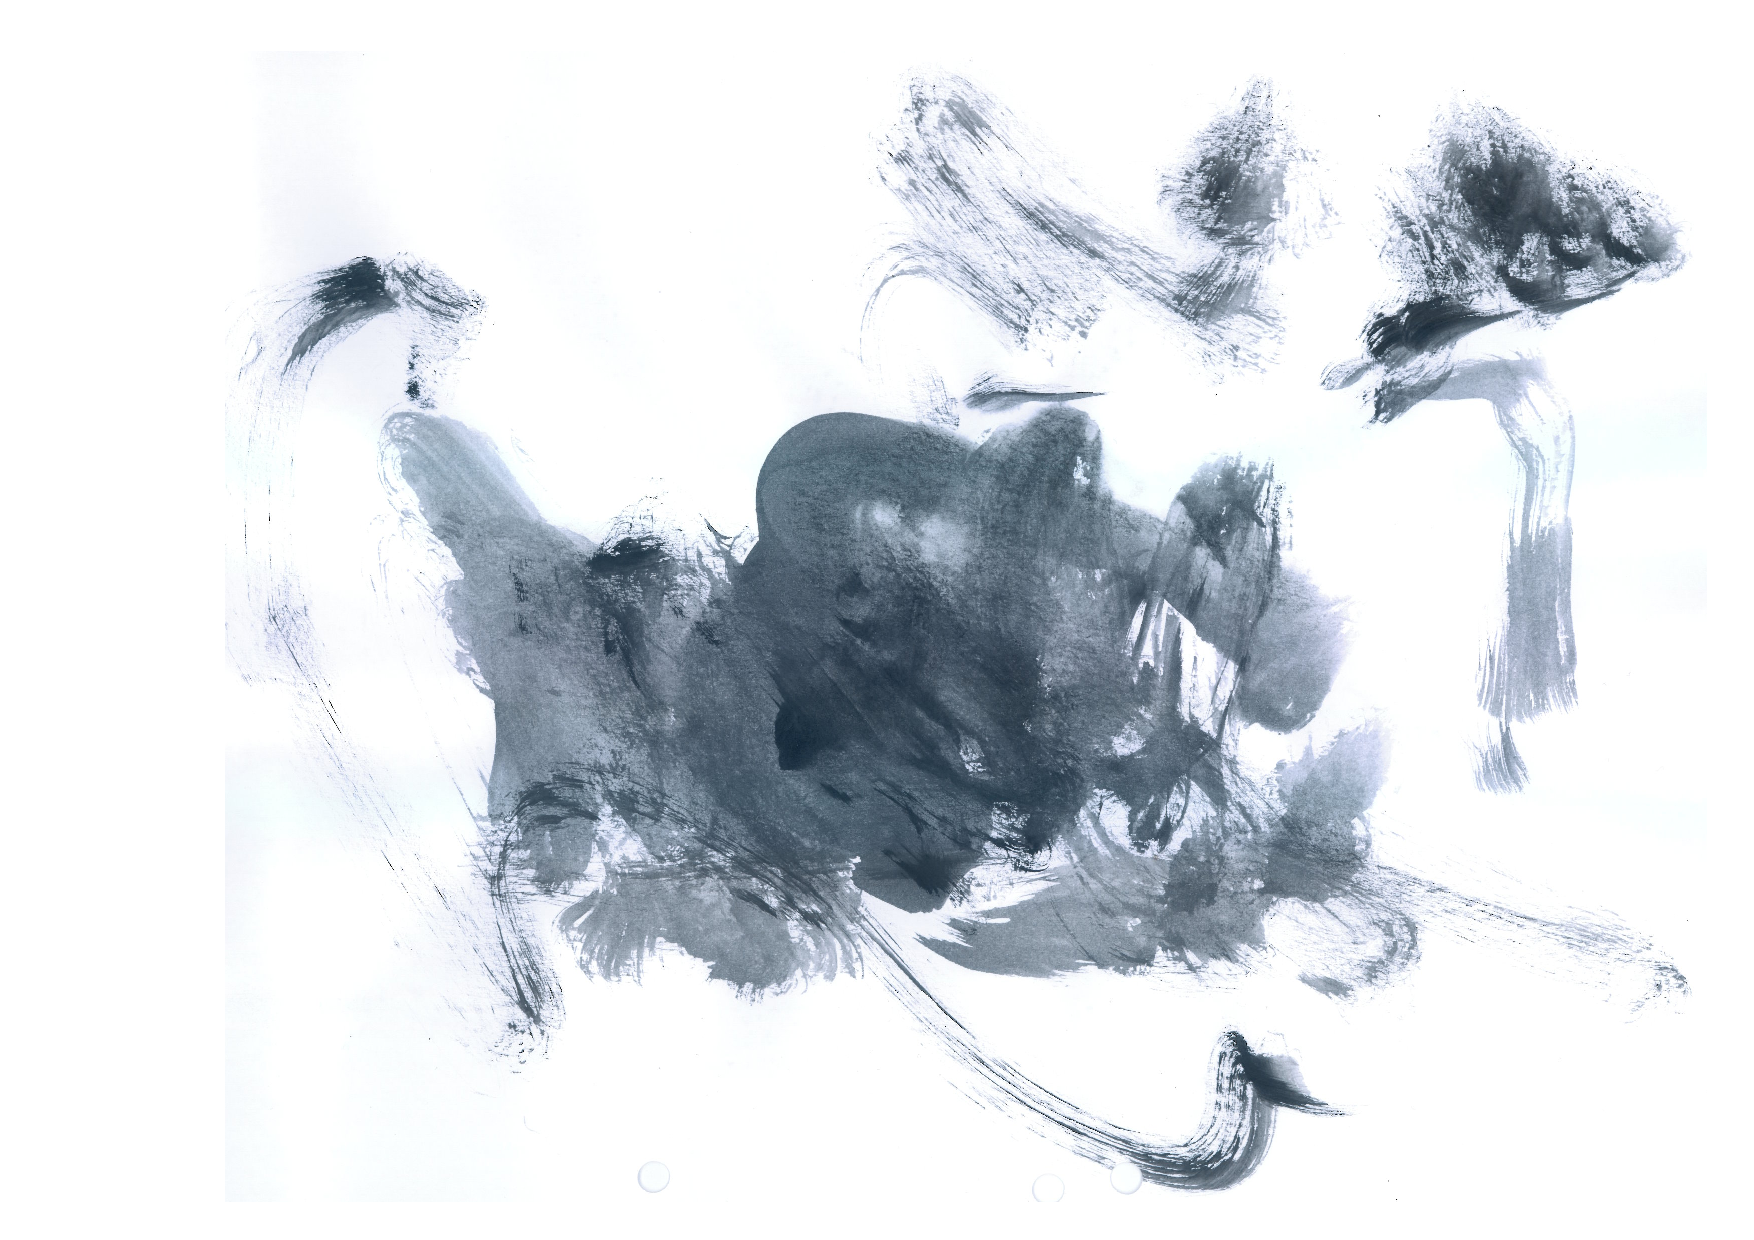
\includegraphics[width=\textwidth]{bilder/dark2.pdf}
    \end{figure}
    \clearpage
}

In all dem Chaos und der Angst hatte nur ein Mädchen keine Angst: Onta. Onta war schon blind geboren worden, ihre fehlte das Licht also nicht. Sie wusste genau wie viele Schritte es vom Tisch bis zur Tür und von dort bis überall hin im Dorf waren. Sie konnte sogar im Wald rennen, so genau hatte sie sich eingeprägt, wo welcher Baum stand. Es dauerte ein paar Tage, bis ihr klar wurde, dass nur sie jetzt noch helfen konnte.

Und so machte sich Onta auf den Weg, den Guhl zu suchen, um ihn zu besänftigen. Wie das gelingen könnte, wusste sie selbst noch nicht so genau. 

Noch nie hatte sie den Wald so leise erlebt. Um so weiter sie kam, um so vorsichtiger musste sie sich den Weg ertasten. Aber sie wusste, dass sie auf dem richtigen Weg war, denn der Gestank des Guhl wurde von Stunde zu Stunde stärker. Nach ungefähr einem Tag Wanderung war sie sicher, am Ziel zu sein. Der Guhl musste jetzt ganz in der Nähe sein.

Onta setzte sich auf einen Stein und wartete. Um sich die Zeit zu vertrieben und gegen die Angst und die Stille nahm sie ihre kleine geschnitzte Flöte und spielte ein Lied. Plötzlich stand der Guhl hinter ihr. Onta konnte ihn spüren. Er musste riesig sein. Niemand wusste genau, wie so ein Guhl aussieht, vielleicht ein bisschen wie ein riesiger Bär. Jedenfalls brummte er wie einer, bloss sehr viel lauter. Aber Onta merkte, dass nichts Böses in diesem Brummen lag. 

Den Geräuschen nach hatte sich der Guhl auf den Boden gesetzt. Onta spielte einfach weiter und immer weiter. Das Brummen des Guhl war gleichmässiger geworden und einem Schnarchen gewichen. Der Guhl war wieder eingeschlafen. Onta spielte weiter so lange sie konnte. Es könnte ein Tag gewesen sein oder zwei, als sie das leise Knacken von Zweigen hinter sich hörte.

Mit ganz leiser Stimme flüsterte eine Stimme ihren Namen. Da hörte Onta auf zu spielen, der Guhl schlief weiter. Die Stimme gehörte einer Jägerin des Dorfes, die sie suchen gekommen war. Als der Guhl eingeschlafen war, war auch das schwarze Licht verschwunden. Onta hatte dies noch nicht bemerkt, da bis hier noch keine Vögel zurückgekehrt waren.

Die Menschen des Dorfes bauten eine grosse Mauer um den Guhl. Nicht um ihn einzusperren, das wäre unmöglich gewesen, sondern um seinen Schlaf zu schützen. Da liegt er noch heute, aber niemand weiss mehr, wo genau das gewesen ist. \end{swb}\hfill {\color{DeepPink}\decofourleft}
